%%% In this section, you will describe all of the various artifacts that you will generate and maintain during the project life cycle. Describe the purpose of each item below, how the content will be generated, where it will be stored, how often it will be updated, etc. Replace the default text for each section with your own description. Reword this paragraph as appropriate.

\subsection{Major Documentation Deliverables}
The major documentation deliverables for this project are project charter, System requirement specification, detailed design specification. Sprint 1 will cover project charter document. The duration for each sprint in this project is 2-weeks long (default length for any new team when assigned the project). The first half of the project is consisting of total number of 4 sprints. First sprint will deliver the project charter. System requirement specification will be delivered the second sprint. Third and fourth sprint will consist of Architectural design specification and detailed design specification including Phase I demo. 

\subsubsection{Project Charter}
This document will be completed by the end of first sprint. As the team makes more progress into the project and adds more components, this document will be altered and updated as required.


\subsubsection{System Requirements Specification}
This document is planned for sprint two. The requirements specifications will be written by the end of second sprint. Since we are following the agile methodology, this document will be modified as required by our sponsor to meet our latest updates. This will be delivered by the end of sprint 2 (October 16, 2023). 

\subsubsection{Architectural Design Specification}
Architectural Design will be initiated in sprint 3. This will be maintained and modified as per the change in the components and the robot arm. This will be delivered by the end of sprint 3 (November 6, 2023). 

\subsubsection{Detailed Design Specification}
Detailed design specifications will be initiated during sprint 5. The document would be altered if the team finds a necessary change. The document will be delivered in the end of sprint 5 (February 12, 2024).

\subsection{Recurring Sprint Items}


\subsubsection{Product Backlog}
Items will be added to backlog based on SRS. These items will be prioritized by the complexity and necessity to reach the goal of the sprint and progress towards end result. Team will use excel to track the backlog. These backlogs will be discussed in meetings. 

\subsubsection{Sprint Planning}
Each sprint will be planned after the termination of previous sprint. There are going to be a total of 8 sprints (Senior Design I has 4 sprints and Senior Design II has 4). 

\subsubsection{Sprint Goal}
The team will decide collaboratively about the sprint goal.  

\subsubsection{Sprint Backlog}
The teams will determine which task or tasks will make it to backlog. 

\subsubsection{Task Breakdown}
Different tasks will be assigned to team members. The task can have a sub team of 2-3 members working on it or it can also be assigned to an individual team member depending upon the complexity of the task. 

\subsubsection{Sprint Burn Down Charts}
The team will decide the burn down charts. This will use MS-Excel. 

\begin{figure}[h!]
    \centering
    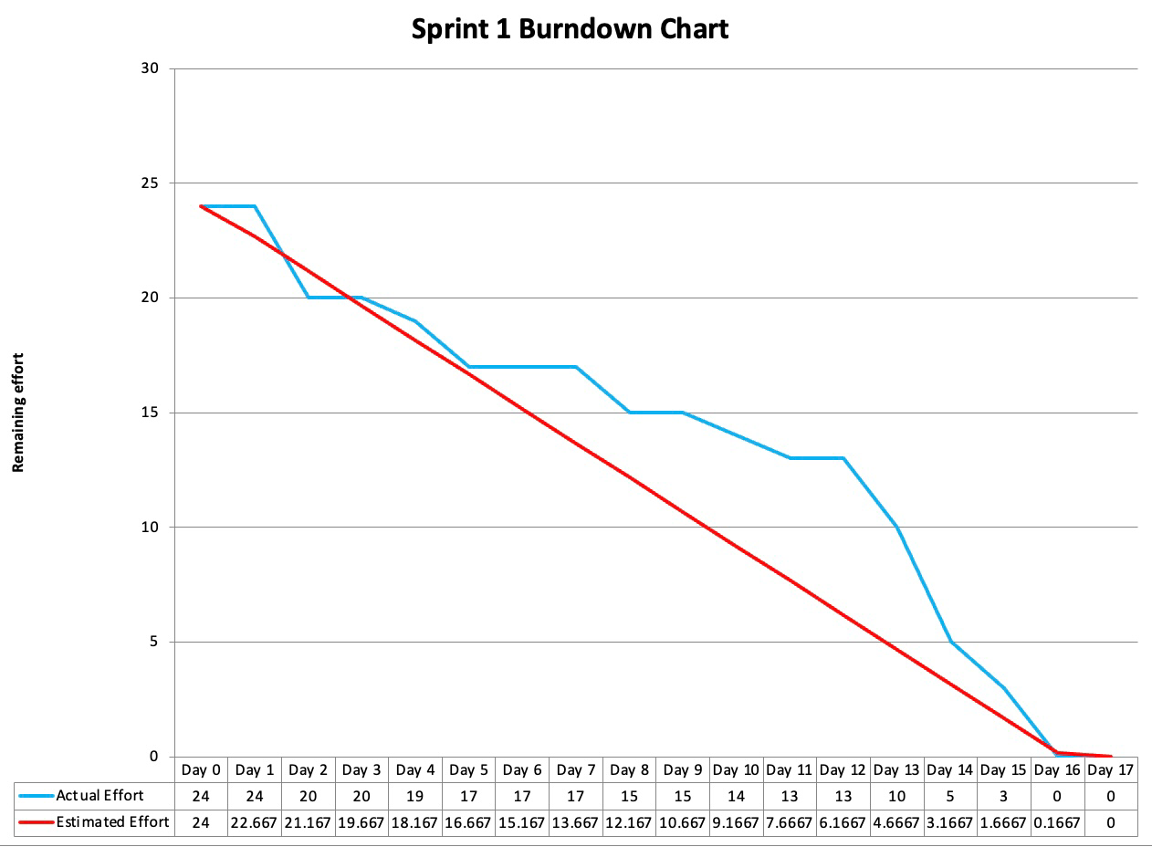
\includegraphics[width=0.5\textwidth]{images/burndown_example2.png}
    \caption{Example sprint burn down chart}
\end{figure}

\subsubsection{Sprint Retrospective}
The retrospective will be handled after carrying out a conversation regarding the previous sprint. Individuals are required to report any sort issues and inconvenience before the sprint end so that important measure can be taken before the sprint ends. Lastly, next sprint goals and previous sprint\'s incompletion (if any) will be discussed before the start of new sprint.  

\subsubsection{Individual Status Reports}
An individual must report the progress that was being through the sprint which will also be recorded. Peer Review will ensure that the team is in the best possible way of communications and are good aware of the other members strengths and weaknesses regarding this project. 

\subsubsection{Engineering Notebooks}
Engineering notebooks will not be used. 

\subsection{Closeout Materials}

\subsubsection{System Prototype}
The final system prototype will include a working RV8 robot arm with a linear rail. This will be demonstrated through a video as well as in the lab where it is setup. 

\subsubsection{Project Poster}
The project poster will discuss the system overview of the project. The overview will include the design and architectural details. It will be delivered after the system prototype is ready. 

\subsubsection{Web Page}
The project webpage will be public and provide access to the documentation associated with the prototype such as project charter, SRS and ASD. This webpage will be updated throughout the project as the sprints will be put to finish. 

\subsubsection{Demo Video}
The demo video will be a source to display the use of the prototype and the purpose the prototype. 

\subsubsection{Source Code}
GitHub will be used as the repository to maintain and store code for this project. All the changes made will be pushed to GitHub. Using GitHub will give us the option to revert if any complication arises. Since the prototype is designed for specific purpose only, the code will be implemented. 

\subsubsection{Source Code Documentation}
The documentation will be provided in a PDF format. 

\subsubsection{Hardware Schematics}
This will be decided during ASD. 

\subsubsection{CAD files}
The prototype will contain a gripper. The team will try to obtain from external retailer. In case of unavailability of the part or if it is unsuited then the teams will use Inkscape to generate CAD files for the gripper and will use it to generate the gripper as designed. 

\subsubsection{Installation Scripts}
The customer will not be required to deploy any software as the team will deploy the software for them. There will be no updates in future for this project. Because this project is only required to fulfill certain task only. 

\subsubsection{User Manual}
The customer will be provided with a digital (PDF) and a printed manual for the project. 